\chapter{Gestion du projet}

\section{outils de gestion utilisés}

Gérer un groupe de projet de sept personnes est évidemment assez complexe, nous avons donc utilisé plusieurs outils pour nous aider. Après la séparation en deux groupes, certains outils ont été abandonnés car ils n'était plus très interessant.

\subsection{Gestionnaire de version}

Nous avons utilisé le gestionnaire de version git pour notre projet. Le gestionnaire permettant la création de branches et leur fusion de façon simple et automatique, nous avons eu l'idée d'utiliser git pour organiser le projet par branche. Une branche de base stable devait servir de version de référence, à partir de laquelle chacun crée sa propre branche de développement. Les branches devaient être fusionnées une fois les développement principaux terminés. Cette organisation permettait d'individualiser les développements ; elle a le mérite d'être sûre, mais elle s'est révelée peu efficace : les branches mettant trop de temps à être fusionnées, la branche de départ est restée longtemps vide, ralentissant la circulation d'information et la mise au point entre les modules dépendants. Par la suite et renforcé par la réduction d'effectif, nous avons rassemblé tous les développements dans une unique branche de développement, fonctionnement simple mais qui s'est révélé suffisant pour nos besoins. 

\subsection{Gestion des ressources}

Lors de la première partie du projet, nous avons utilisé le logiciel planner pour faire un diagramme de gantt. Ce planning initial a permis de mettre en évidence les principales taches, leur découpage en modules, et les premières attributions de tâche. Ce logiciel est assez interessant car il permettait de rassembler le planning, l'attribution des tâches et l'avancement constaté dans un seul fichier, de manière simple et complète. 
Nous avons abandonné cet outil dans la deuxième partie du projet car, à quatre, il était aussi simple de se répartir les taches oralement. L'ajustement de répartition par rapport à l'avancement réel en a été facilité.

\section{Mode de développement}

Nous avons adoptés un cycle de développement en "V", avec des rencontres régulières avec le client. Nous avons fait dans la mesure du possible les tests unitaires de chaques modules. La principale difficulté a été la mise en place de test d'intégration, le fonctionnement des modules n'étant pas toujours facilement observable. Le développement des modules s'est pour la plupart fait à deux codeurs.

\begin{tabular}{c}
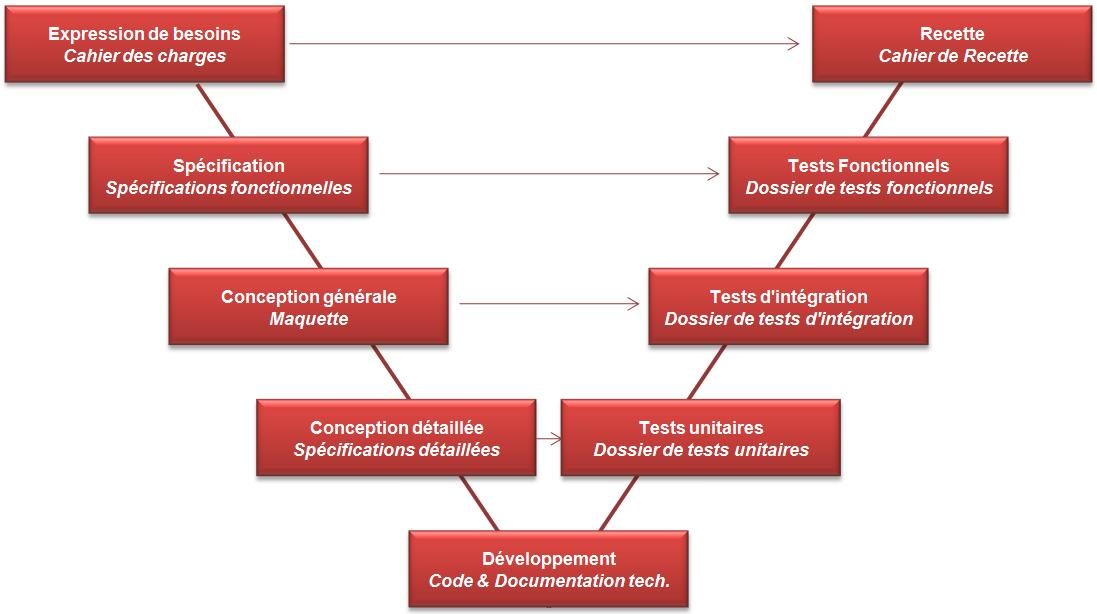
\includegraphics[width=140mm]{Images/Cycle_en_V.jpg}
\end{tabular}{c}
